\part{Industrielt Netværk}
\chapter{Introduktion til Industrielle Netværk}
\label{chapter:introduktion_industrielle_netværk}
\section{Hvad er Industrielt Netværk?}
Industrielle netværk refererer til kommunikationssystemer designet specifikt til at forbinde enheder i industrielle miljøer som fabrikker, produktionsanlæg og andre automatiserede systemer. Disse netværk muliggør dataudveksling mellem forskellige maskiner og kontrolsystemer, hvilket optimerer produktionsprocesser, forbedrer effektiviteten og øger pålideligheden.

\subsection{Historisk Udvikling af Netværk i Industrien}
Industrielle netværk har gennemgået en betydelig udvikling over tid. I begyndelsen blev industrielle kontrolsystemer typisk isolerede og brugte proprietære kommunikationsprotokoller. Med fremkomsten af standardiserede protokoller og netværksteknologier som Ethernet og TCP/IP, er det blevet muligt at integrere industrielle netværk med virksomhedens IT-systemer, hvilket har ført til mere sammenhængende og fleksible produktionsmiljøer.

\subsection{Tidlige Industrielle Netværk}
I de tidlige dage af industriel automatisering var kommunikationssystemer ofte punkt-til-punkt forbindelser, hvor hver enhed var direkte forbundet med kontrolsystemet. Dette resulterede i komplekse og dyre installationer, der var svære at vedligeholde og udvide.

\subsection{Overgang til Standardiserede Protokoller}
Med introduktionen af standardiserede protokoller som Modbus og PROFIBUS i 1980'erne, blev det muligt at oprette mere fleksible og skalerbare netværk. Disse protokoller gjorde det lettere at forbinde enheder fra forskellige producenter og reducere kompleksiteten i installationsprocessen.

\subsection{Integration med Ethernet og IT-Systemer}
I 1990'erne og 2000'erne begyndte industrielle netværk at integrere Ethernet-teknologi, hvilket gjorde det muligt at udnytte de højere hastigheder og den større båndbredde, som Ethernet tilbyder. Dette førte til udviklingen af industri-specifikke Ethernet-protokoller som EtherNet/IP, PROFINET og Modbus TCP. Integration med IT-systemer har desuden gjort det muligt for virksomheder at implementere Industri 4.0-konceptet, hvor produktionsdata kan analyseres i realtid for at optimere driften.

\subsection{Nutidige og Fremtidige Trends}
I dag fortsætter industrielle netværk med at udvikle sig med fokus på trådløse teknologier, cybersikkerhed og Internet of Things (IoT). Fremtidige trends omfatter brugen af 5G til industriel kommunikation, øget brug af kunstig intelligens til netværksovervågning og vedligeholdelse samt integration af avancerede sensorer og aktuatorer for at forbedre produktionsprocesser.

\subsection{Betydningen af Industrielle Netværk}
Industrielle netværk spiller en afgørende rolle i moderne produktionsmiljøer ved at:
\begin{itemize}
	\item \textbf{Forbedre Effektiviteten:} Automatisering og realtidsdataudveksling mellem maskiner og kontrolsystemer optimerer produktionsprocesser og reducerer nedetid.
	\item \textbf{Øge Pålideligheden:} Standardiserede protokoller og robuste netværksdesigns sikrer pålidelig kommunikation selv i krævende industrielle miljøer.
	\item \textbf{Muliggøre Fleksibilitet:} Skalerbare netværk gør det nemmere at tilpasse sig ændringer i produktionskrav og integrere nye teknologier uden omfattende ændringer i infrastrukturen.
	\item \textbf{Styrke Sikkerheden:} Avancerede sikkerhedsprotokoller og netværksovervågning beskytter mod cybertrusler og uautoriseret adgang.
\end{itemize}

\chapter{Protokoller og Elektriske Standarder}

\section{Introduktion til Protokoller og Elektriske Standarder}
I industrielle netværk spiller både netværksprotokoller og elektriske standarder en afgørende rolle for at sikre effektiv og pålidelig kommunikation. Selvom disse to begreber ofte nævnes sammen, tjener de forskellige formål og adresserer forskellige aspekter af datakommunikation. Det er derfor vigtigt at forstå deres forskelle og hvordan de komplementerer hinanden.

\section{Netværksprotokoller: Reglerne for Kommunikation}
En netværksprotokol kan sammenlignes med et sprog eller en samtaleetikette, som alle deltagere i en samtale skal følge for at kunne forstå hinanden. Ligesom mennesker har brug for et fælles sprog for at kommunikere effektivt, kræver netværksenheder en fælles protokol for at udveksle data korrekt. En netværksprotokol definerer de regler og konventioner, som netværksenheder skal følge, herunder hvordan data pakkes, adresseres, transmitteres, modtages og behandles.

\subsection{Analogier for at Forstå Netværksprotokoller}
For at forstå netværksprotokoller kan vi bruge analogien med en samtale mellem mennesker. Tænk på netværksprotokollen som de regler, der dikterer, hvordan en samtale skal foregå for at sikre, at begge parter forstår hinanden:

\begin{itemize}
	\item \textbf{Start af Kommunikation:} Ligesom en samtale begynder med en hilsen, starter en netværksforbindelse ofte med en \texttt{TCP connection request}, hvor en enhed anmoder om at etablere en forbindelse. Modparten svarer med en \texttt{TCP connection reply} for at bekræfte.
	\item \textbf{Udveksling af Information:} Under samtalen udveksler parterne information, som spørgsmål og svar, f.eks. "Got the time?" og "2:00". I en netværkskommunikation kunne dette svare til udveksling af data, hvor en enhed sender en kommando, og den anden enhed reagerer med den ønskede information.
	\item \textbf{Afslutning:} Når samtalen er færdig, kan den ene person sige "farvel," ligesom en netværksforbindelse afsluttes ved, at begge parter signalerer, at de er færdige med kommunikationen.
\end{itemize}

\begin{figure}[h]
	\centering
	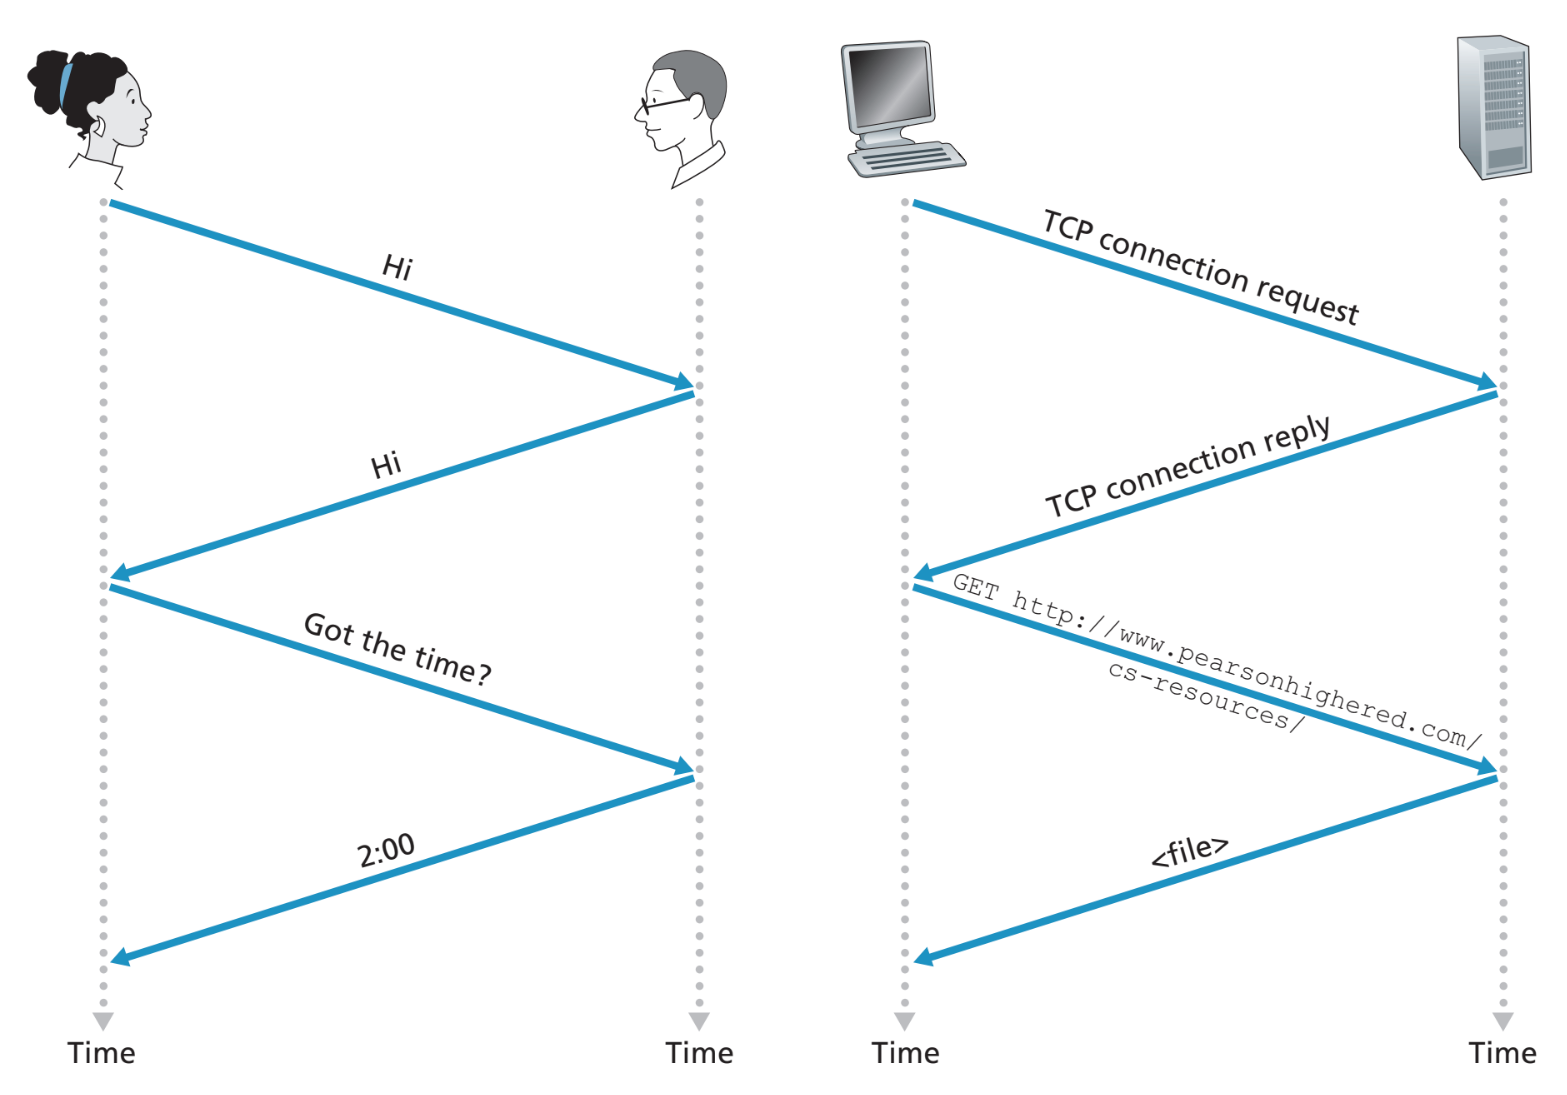
\includegraphics[width=\textwidth]{fig/fig42.png}
	\caption{Sammenligning mellem en menneskelig samtale og en TCP-forbindelse}
	\label{fig:tcp-analogy}
\end{figure}
\noindent Billedet i figur \ref{fig:tcp-analogy} illustrerer, hvordan en sådan kommunikation foregår, både mellem mennesker og i en netværksprotokol som TCP. Denne visuelle analogi hjælper med at forstå, hvordan protokoller sikrer, at begge parter i en netværkskommunikation forstår hinanden korrekt og pålideligt.
\newline\newline\noindent
Eksempler på almindelige netværksprotokoller i industrielle netværk inkluderer Ethernet/IP, Profinet, og Modbus TCP. Disse protokoller muliggør pålidelig kommunikation mellem forskellige enheder såsom PLC'er, sensorer, og aktuatorer i et automatiseret miljø.

\section{Elektriske Standarder: Den Fysiske Infrastruktur}
Mens netværksprotokoller styrer, hvordan data kommunikeres, beskriver elektriske standarder de fysiske egenskaber og specifikationer for, hvordan data transmitteres over et medie. Dette inkluderer alt fra typen af kabler og stik, til spændingsniveauer og frekvenser, der anvendes under transmissionen.

\subsection{Analogier for at Forstå Elektriske Standarder}
Vi kan forstå elektriske standarder ved at sammenligne dem med jernbanespor:

\begin{itemize}
	\item \textbf{Sporbredde:} Ligesom tog skal køre på skinner med en bestemt bredde, skal data overføres gennem kabler med specifikke fysiske egenskaber. Standarderne specificerer, hvilken type kabler (f.eks. kobber eller fiberoptik) og stik der skal bruges.
	\item \textbf{Sikkerhed og Pålidelighed:} Elektriske standarder sikrer, at dataoverførslen er sikker og pålidelig ved at specificere grænser for elektrisk støj og spænding. Dette kan sammenlignes med sikkerhedsforanstaltninger på jernbanen, der forhindrer ulykker og sikrer, at togene kører uden afbrydelser.
	\item \textbf{Båndbredde:} Ligesom jernbanesystemer har kapacitet til at transportere et bestemt antal tog per tidsenhed, dikterer elektriske standarder også, hvor hurtigt data kan overføres og hvor meget information der kan transporteres samtidigt.
\end{itemize}
\noindent
Eksempler på elektriske standarder omfatter RS-232, RS-485, og IEEE 802.3 (Ethernet-standarder). Disse standarder definerer de fysiske parametre, såsom kabeltype og stik, der er nødvendige for at sikre kompatibilitet og pålidelighed i datatransmissionen.

\section{Eksempel på Samspil mellem Protokoller og Elektriske Standarder}
Lad os overveje en situation, hvor en industriel robotarm kommunikerer med en kontrolstation over et netværk. Netværksprotokollen, såsom Profinet, styrer, hvordan data om robotarmens position og status sendes til kontrolstationen og tilbage. Den elektriske standard, såsom Ethernet (IEEE 802.3), bestemmer, hvilken type kabler og stik der bruges, samt de fysiske transmissionsparametre, der sikrer, at dataene overføres korrekt og pålideligt.
\newline\newline\noindent
I denne situation fungerer netværksprotokollen som "sproget", som enhederne bruger til at "tale" med hinanden, mens den elektriske standard fungerer som "infrastrukturen", der gør det muligt for denne kommunikation at finde sted. Begge er nødvendige for at sikre en problemfri og effektiv drift af det industrielle netværk.

\section{Opsummering: Forskellen mellem Protokoller og Elektriske Standarder}
Selvom både netværksprotokoller og elektriske standarder er afgørende for effektiv datakommunikation i industrielle netværk, tjener de forskellige formål:

\begin{itemize}
	\item \textbf{Netværksprotokoller:} Disse styrer, hvordan data pakkes, sendes, modtages, og behandles mellem enheder på et netværk. De skaber et fælles sprog, som alle enheder i netværket forstår, og sikrer, at informationen overføres korrekt.
	
	\item \textbf{Elektriske Standarder:} Disse definerer de fysiske parametre for datatransmissionen, herunder kabeltyper, spændingsniveauer og forbindelsesmåder. De sikrer, at de tekniske aspekter af dataoverførslen er sikre og pålidelige, hvilket muliggør kompatibilitet mellem forskellige enheder og systemer.
\end{itemize}
\noindent Protokollerne kan ses som de "regler" og "sprog", som enhederne i netværket bruger til at kommunikere, mens de elektriske standarder er den "infrastruktur", der muliggør, at denne kommunikation kan foregå sikkert og effektivt. For at opnå en robust industriel netværksløsning er det nødvendigt at anvende både passende protokoller og elektriske standarder i designet og implementeringen.

\chapter{Netværkstopologi}
\begin{figure}[!h]
	\centering
	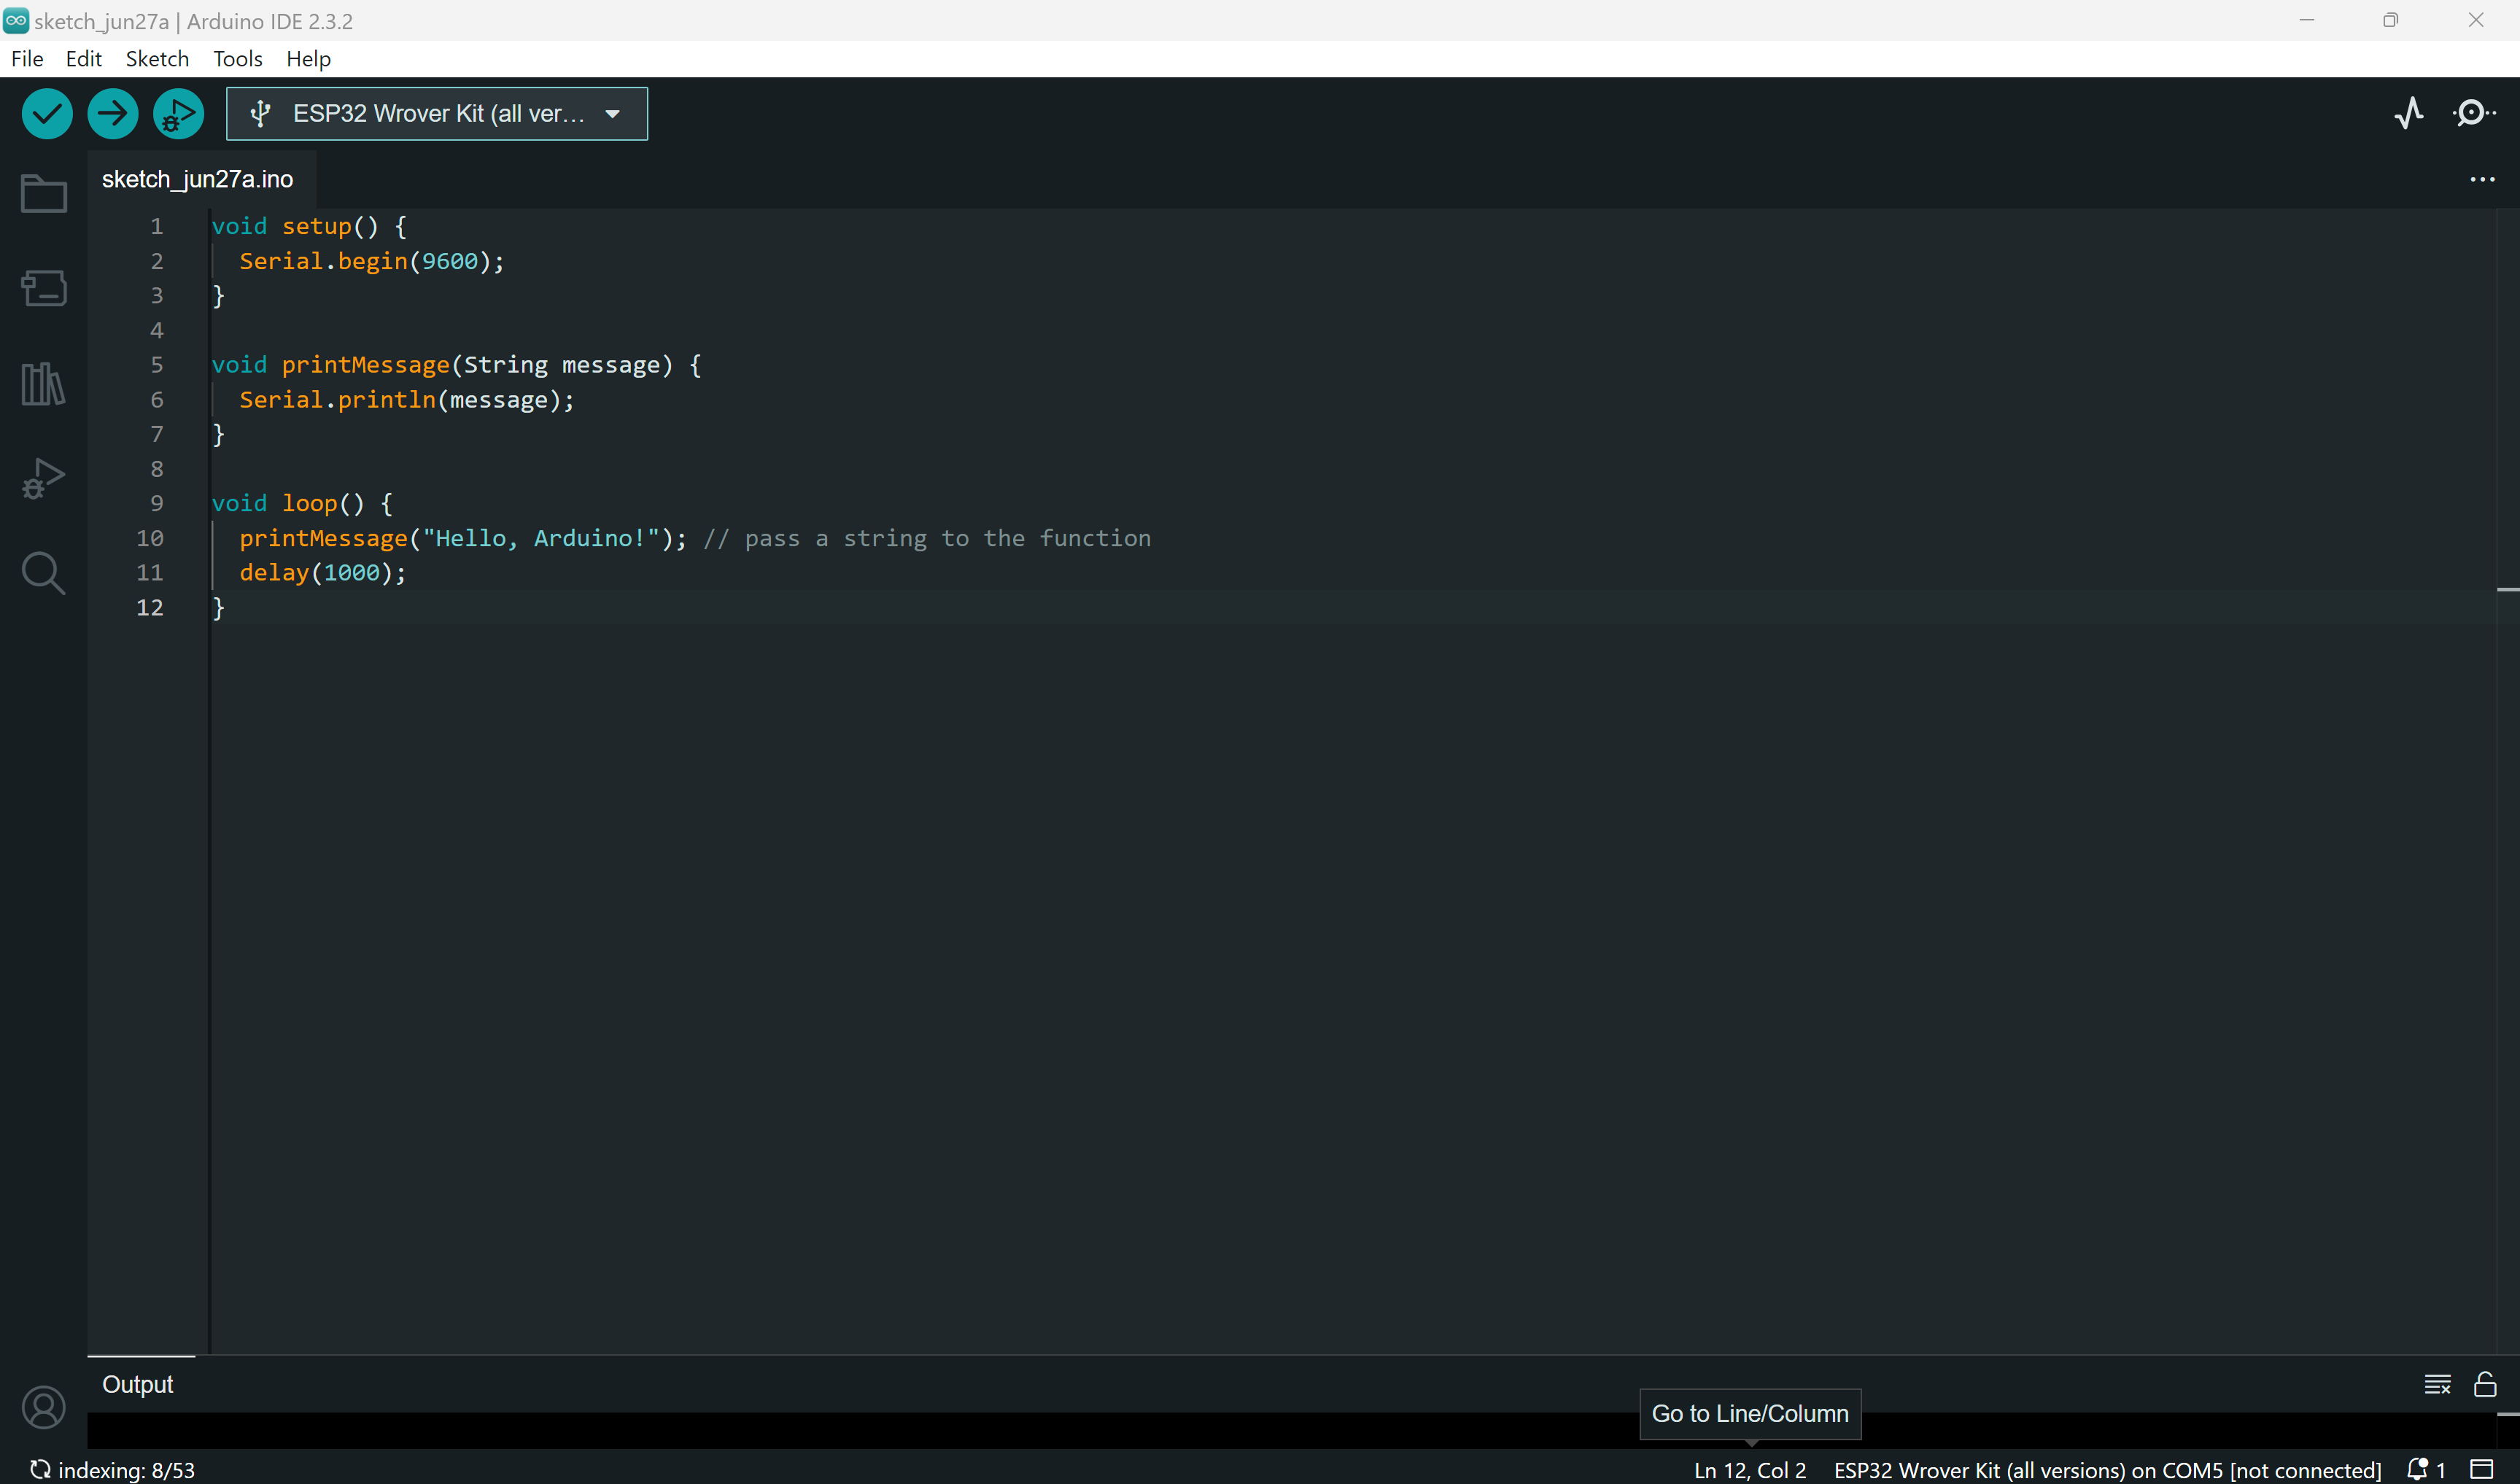
\includegraphics[width=\linewidth]{fig/fig12.png}
	\caption{Netværkstopologi}
\end{figure}
\noindent Netværkstopologi refererer til arrangementet og layoutet af noder og forbindelser i et netværk. Det beskriver både den fysiske og logiske struktur af netværket. Der er flere forskellige typer af topologier, hver med sine egne fordele og ulemper. Nedenfor gennemgås de mest almindelige netværkstopologier:

\section{Punkt-til-punkt Topologi}
I en punkt-til-punkt topologi er to noder direkte forbundet til hinanden. Denne type topologi bruges ofte i situationer, hvor en direkte forbindelse mellem to enheder er nødvendig.
\begin{itemize}
	\item \textbf{Fordele:}
	\begin{itemize}
		\item Meget enkel og hurtig forbindelse.
		\item Lav latenstid og høj båndbredde.
	\end{itemize}
	\item \textbf{Ulemper:}
	\begin{itemize}
		\item Ikke skalerbar; kun egnet til små netværk.
		\item Hvis forbindelsen fejler, går kommunikationen tabt.
	\end{itemize}
\end{itemize}

\section{Bustopologi}
I en bustopologi er alle noder forbundet til en enkelt kommunikationslinje eller bus. Dataene, der sendes af en node, rejser langs bussen og kan modtages af alle noderne.
\begin{itemize}
	\item \textbf{Fordele:}
	\begin{itemize}
		\item Nem og billig at installere.
		\item Kræver mindre kabel end en stjernetopologi.
	\end{itemize}
	\item \textbf{Ulemper:}
	\begin{itemize}
		\item Svært at fejlfinde og identificere problemer.
		\item Begrænset kabel længde og antal noder.
		\item Hvis hovedkabel fejler, går hele netværket ned.
	\end{itemize}
\end{itemize}

\section{Ringtopologi}
I en ringtopologi er noderne forbundet i en cirkulær rækkefølge. Hver node har præcis to naboer, og data bevæger sig i én retning (eller i nogle tilfælde i begge retninger) langs ringen.
\begin{itemize}
	\item \textbf{Fordele:}
	\begin{itemize}
		\item Dataoverførsel er relativt hurtig, da data bevæger sig i en bestemt retning.
		\item Ingen kollisionsdomæner som i bustopologi.
	\end{itemize}
	\item \textbf{Ulemper:}
	\begin{itemize}
		\item En fejl i en enkelt node eller forbindelse kan påvirke hele netværket.
		\item Mere kompleks at installere og konfigurere.
	\end{itemize}
\end{itemize}

\section{Stjernetopologi}
I en stjernetopologi er alle noder forbundet til en central hub eller switch. Hubben fungerer som en repeater for dataene, hvilket betyder, at data, der sendes fra en node, først sendes til hubben og derefter videre til den destination, der er tiltænkt.
\begin{itemize}
	\item \textbf{Fordele:}
	\begin{itemize}
		\item Enkel at installere og administrere.
		\item Fejl i en enkelt kabel påvirker ikke resten af netværket.
		\item Let at tilføje eller fjerne noder uden at forstyrre netværket.
	\end{itemize}
	\item \textbf{Ulemper:}
	\begin{itemize}
		\item Hvis central hub fejler, går hele netværket ned.
		\item Kræver mere kabel end nogle andre topologier.
	\end{itemize}
\end{itemize}

\section{Trætopologi}
Trætopologi, også kendt som hierarkisk topologi, er en hybrid topologi, der kombinerer egenskaberne af stjernetopologi og bustopologi. Den består af grupper af stjernetopologier, der er forbundet til et bus-lignende backbone-kabel.
\begin{itemize}
	\item \textbf{Fordele:}
	\begin{itemize}
		\item Udvidelsesvenlig og let at administrere.
		\item Fejl i en enkelt node påvirker ikke hele netværket.
	\end{itemize}
	\item \textbf{Ulemper:}
	\begin{itemize}
		\item Mere kompleks at konfigurere end en simpel stjerne- eller bustopologi.
		\item Backbone-kablet er et enkelt fejlpunkt.
	\end{itemize}
\end{itemize}

\section{Masketopologi}
I en masketopologi er hver node forbundet til flere andre noder, hvilket skaber et netværk af forbindelser. Dette kan være en fuld mesh, hvor alle noder er forbundet til hinanden, eller en delvis mesh, hvor nogle noder kun er forbundet til nogle få andre noder.
\begin{itemize}
	\item \textbf{Fordele:}
	\begin{itemize}
		\item Meget pålidelig, da flere forbindelser sikrer, at data kan tage alternative ruter.
		\item Fejl i en enkelt forbindelse påvirker ikke hele netværket.
	\end{itemize}
	\item \textbf{Ulemper:}
	\begin{itemize}
		\item Meget dyrt og komplekst at installere og vedligeholde.
		\item Kræver mange kabler og porte.
	\end{itemize}
\end{itemize}

\section{Hybridtopologi}
En hybridtopologi er en kombination af to eller flere forskellige typer af netværkstopologier. Denne type topologi anvendes ofte i store netværk, hvor det er nødvendigt at udnytte fordelene ved flere forskellige topologier.
\begin{itemize}
	\item \textbf{Fordele:}
	\begin{itemize}
		\item Fleksibel og skalerbar.
		\item Kan optimeres for at udnytte styrkerne ved flere topologier.
	\end{itemize}
	\item \textbf{Ulemper:}
	\begin{itemize}
		\item Kompleks at designe og implementere.
		\item Højere omkostninger ved installation og vedligeholdelse.
	\end{itemize}
\end{itemize}

\section{Daisy Chain Topologi}
I en daisy chain topologi er hver node forbundet til to andre noder, og danner en lineær kæde. Denne type topologi bruges ofte i små netværk eller til at forbinde enheder i en sekventiel rækkefølge.
\begin{itemize}
	\item \textbf{Fordele:}
	\begin{itemize}
		\item Enkel og billig at installere.
		\item Kræver mindre kabel end andre topologier.
	\end{itemize}
	\item \textbf{Ulemper:}
	\begin{itemize}
		\item Dataoverførsel kan være langsommere, da data skal passere gennem flere noder.
		\item Hvis en node i midten af kæden fejler, kan det bryde kommunikationen i netværket.
	\end{itemize}
\end{itemize}
\noindent Valget af netværkstopologi afhænger af flere faktorer, herunder netværkets størrelse, budget, ønsket pålidelighed og krav til datahastighed. Forståelsen af de forskellige topologier og deres egenskaber er afgørende for at kunne designe og implementere effektive netværksløsninger.
\clearpage